\subsubsection{Simulation}

The simulation is a \texttt{discrete-time simulation}, where each tick represents an amount of time that has passed.
This allows to control the \texttt{delta time}, therefore allowing to speed up/down the simulation.

Any component that requires to update its state in steps and know how much time
has passed will implement the interface \texttt{DiscreteObject}.

\begin{figure}[H]
\centering{}
% 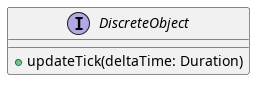
\includegraphics[width=\textwidth,height=\textheight,keepaspectratio]{magnani/uml/discreteobject.png}
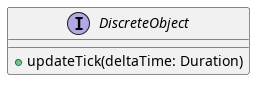
\includegraphics[keepaspectratio]{magnani/uml/discreteobject.png}
\caption{UML diagram of the DiscreteObject interface}
\label{magnani:uml:discreteobject}
\end{figure}

\paragraph{Problem} Since the simulation can be sped up, we have to track the time in the simulation environment
\paragraph{Solution} Creation of the concept of \texttt{Clock} that stores the time and is updated at each tick.

\begin{figure}[H]
\centering{}
% 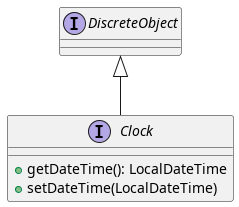
\includegraphics[width=\textwidth,height=\textheight,keepaspectratio]{magnani/uml/clock.png}
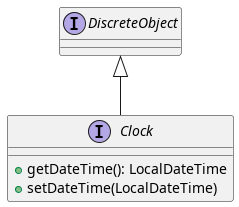
\includegraphics[keepaspectratio]{magnani/uml/clock.png}
\caption{UML diagram of the clock}
\label{magnani:uml:clock}
\end{figure}

\subsubsection{Control of the simulation}

The game loop is handled in the simulation manager.

The simulation manager logic is split between the \texttt{SimManager} and \texttt{SimManagerViewObserver}.

Any \texttt{DiscreteObject} can ask to be updated by the game loop with the
\texttt{Observer} pattern,via the \texttt{SimManager} method \texttt{addObserver}.

The simulation manager interfaces with its view counterpart to allow pause/resume
and time rate control via the \texttt{SimManagerViewObserver} using the \texttt{Observer} pattern.

\begin{figure}[H]
\centering{}
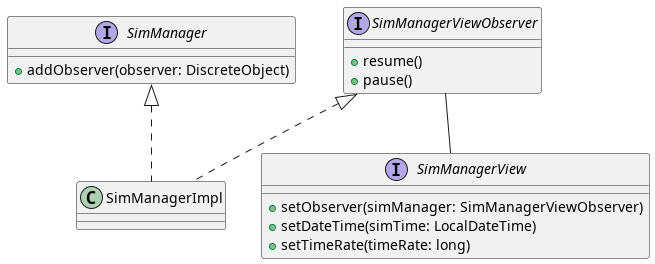
\includegraphics[width=\textwidth,height=\textheight,keepaspectratio]{magnani/uml/simmanager.png}
\caption{UML diagram of the SimulationManager}
\label{magnani:uml:simmanager}
\end{figure}
